\documentclass[class=article, crop=false]{standalone}

\begin{document}
\section{Partie 5 - Observateur - Contrôleur}
On va maintenant utiliser l'état estimé par l'observateur dans le retour d'état. La loi de commande est donc de la forme:
\begin{equation}
    u(t) = u_{\text{ref}} - K \underbrace{(\hat{X}(t) - X_{\text{ref}})}_{\delta \hat{X}(t)}
\end{equation}
On pourra choisir le gain $K$ calculé en plaçant les valeurs propres en boucle fermée ou en minimisant le critère $J_{LQ}$.

\newpage
\subsection{Question 23}
\begin{exercise}
    Implémenter l'observateur-contrôleur dans le modèle Simulink. Vérifier qu'il permet bien d'estimer l'état et de stabiliser la Balle sur la position $r_{\text{ref}} = 0$ avec un état initial suffisamment proche de l'équilibre pour que le linéarisé tangent reste une approximation valable.
\end{exercise}
\begin{resolution}
    L'Observateur Contrôleur complet peut être implémente avec le diagramme Simulink suivant:
    \begin{figure}[H]
        \centering
        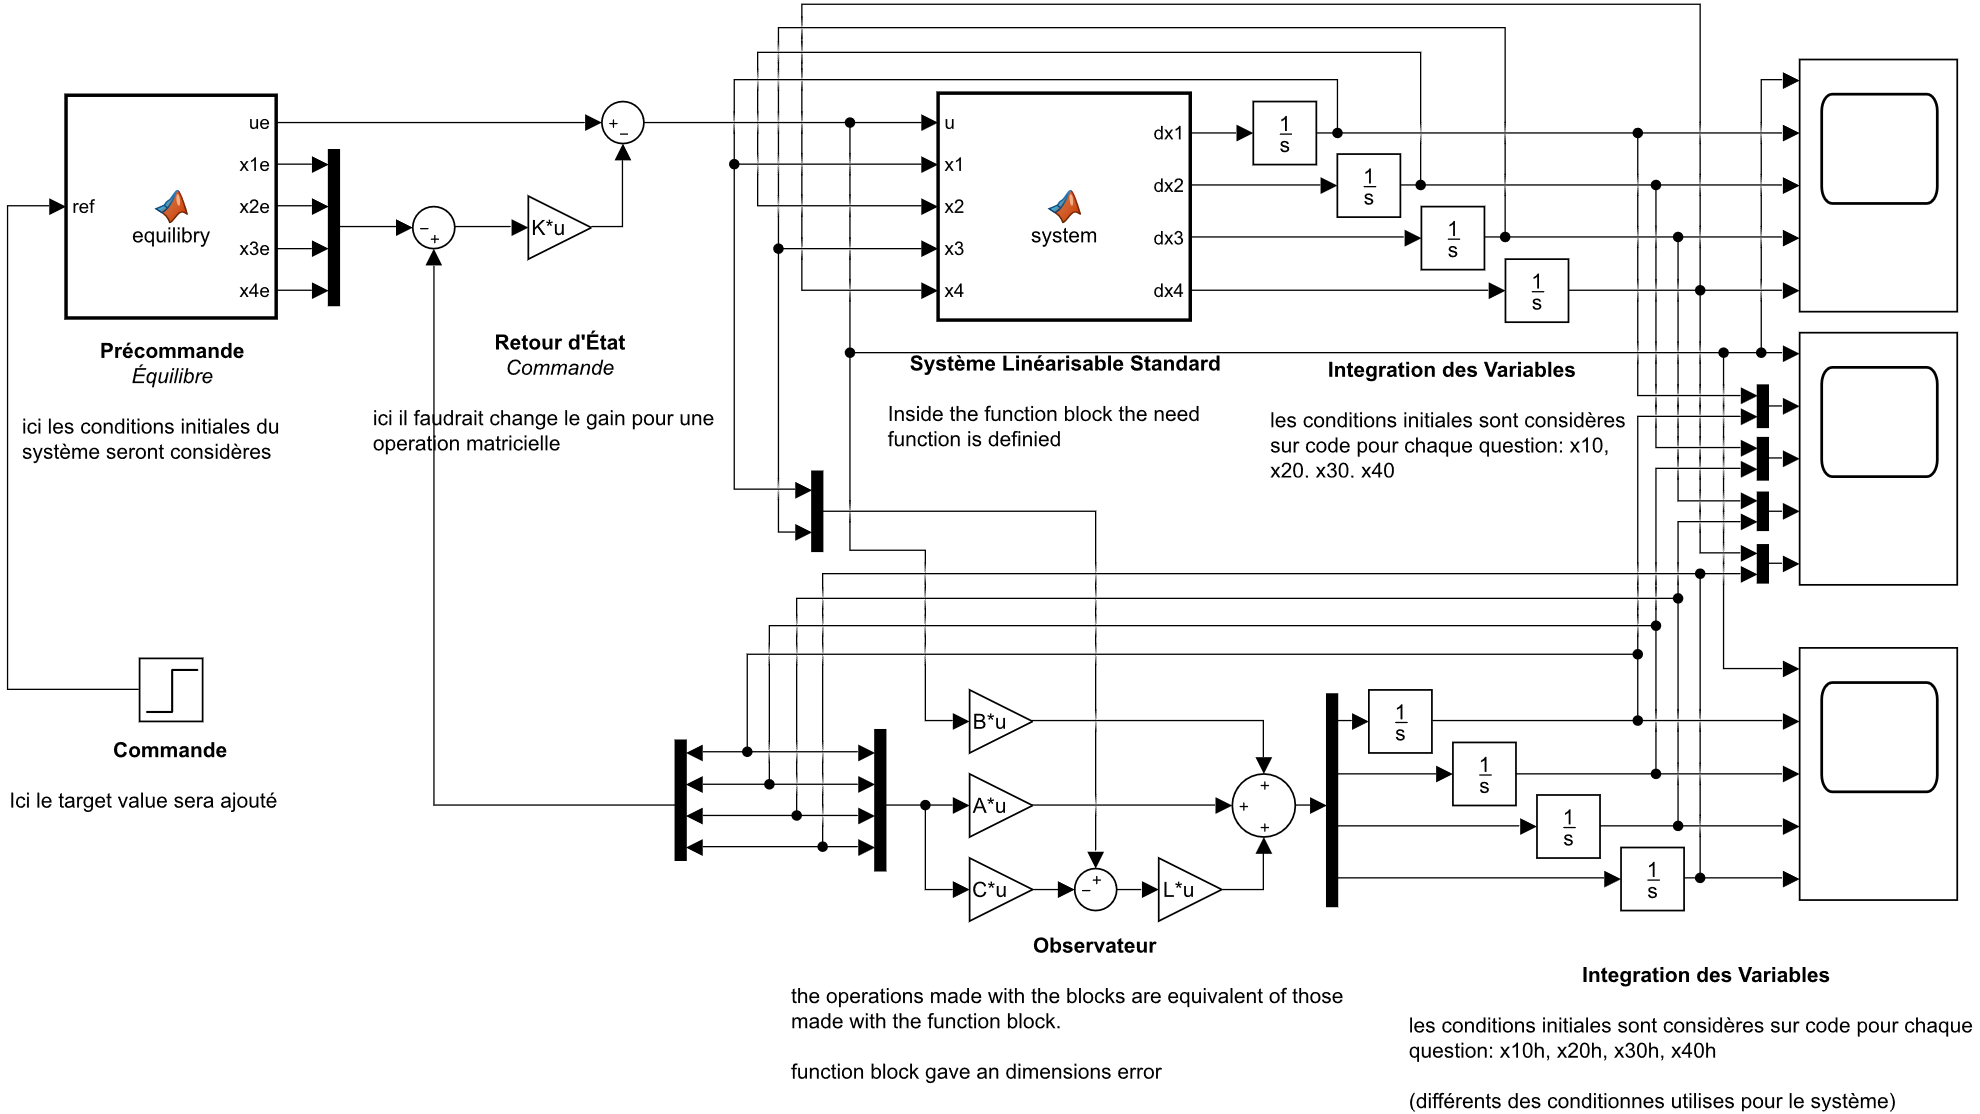
\includegraphics[width=0.7\textwidth]{../images/system_simulink_5.png}
        \caption{Système d'intérêt Simulink, Observateur Contrôleur}
    \end{figure}
    Qui donne les résultats suivants:
    \begin{figure}[H]
        \centering
        \begin{subfigure}[b]{0.45\textwidth}
            \centering
            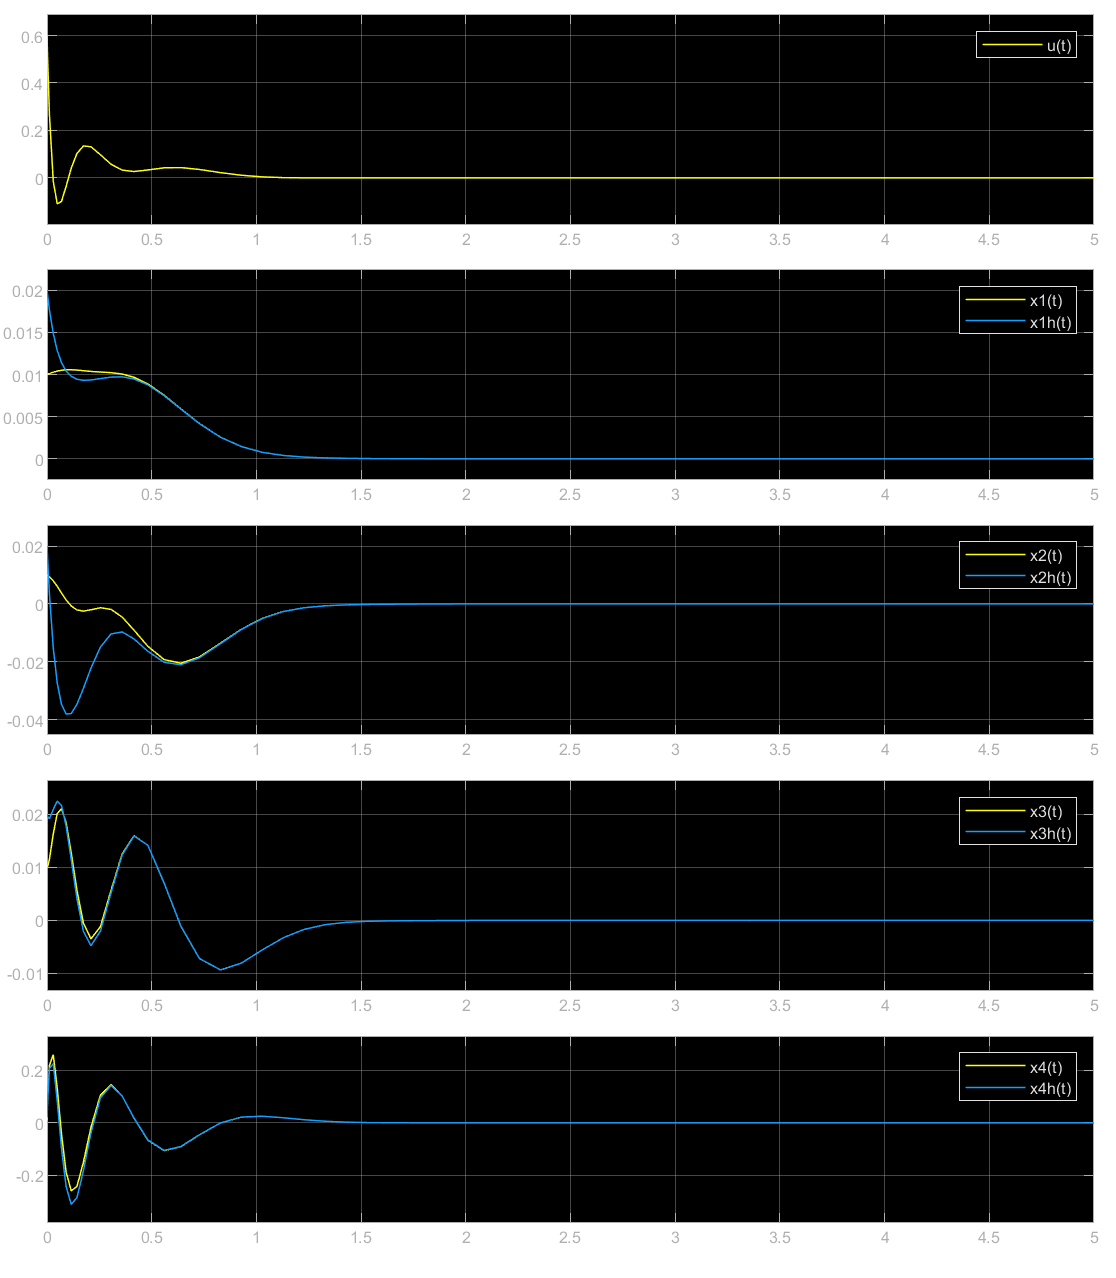
\includegraphics[width=\textwidth]{../images/m5_r0_s0.01_o0.02.png}
            \caption{$x_1(0) = x_2(0) = 0.01$ et $\hat{x}_1(0) = \hat{x}_2(0) = 0.02$}
        \end{subfigure}
        \begin{subfigure}[b]{0.45\textwidth}
            \centering
            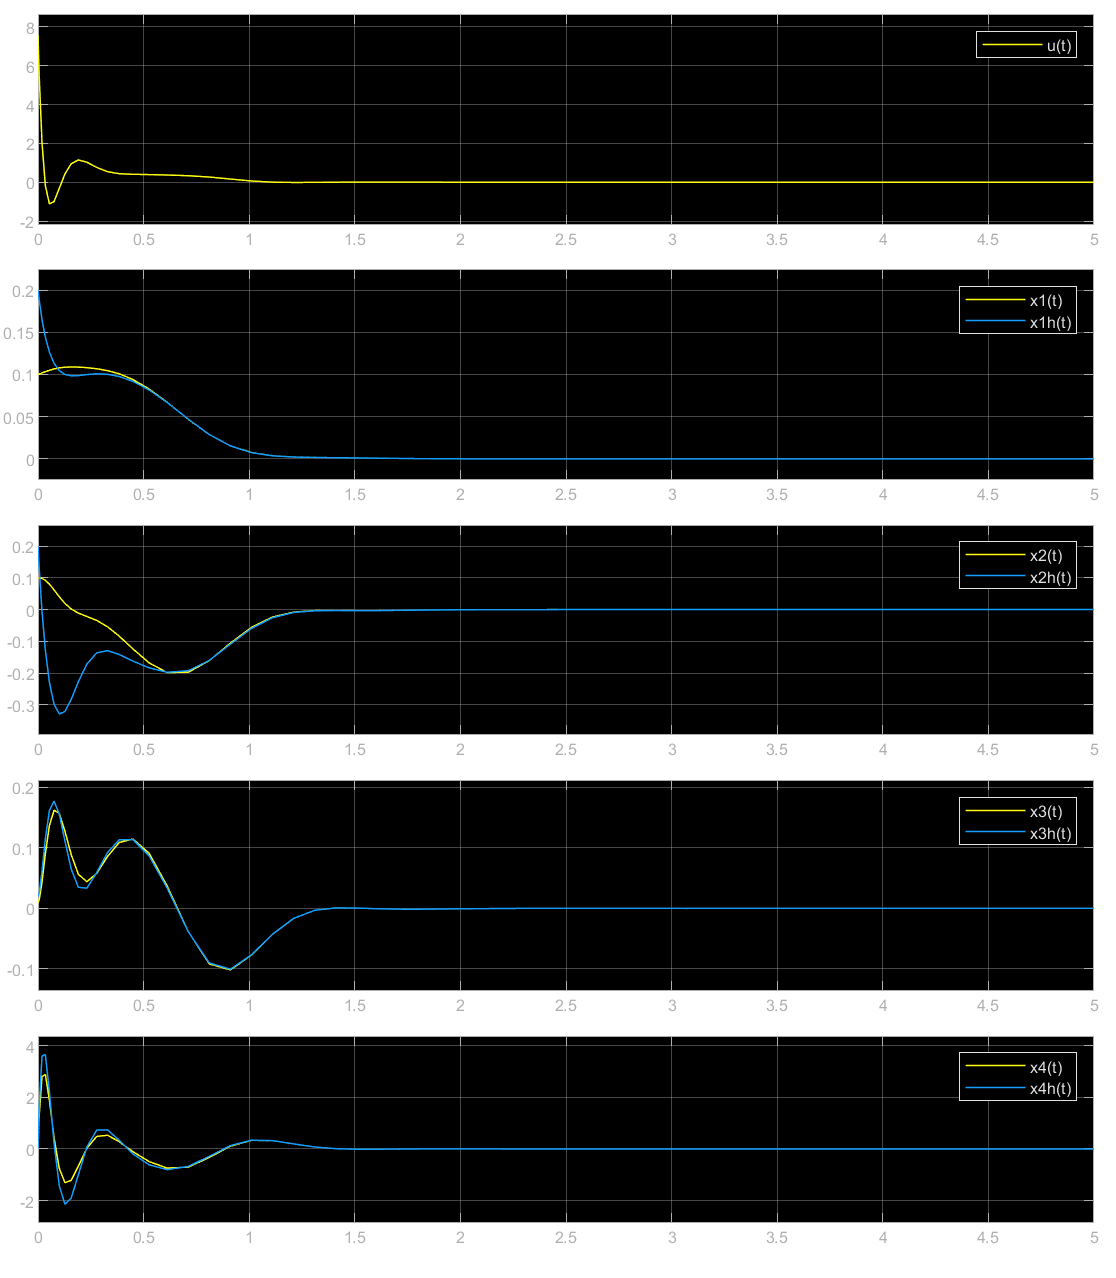
\includegraphics[width=\textwidth]{../images/m5_r0_s0.1_o0.2.png}
            \caption{$x_1(0) = x_2(0) = 0.1$ et $\hat{x}_1(0) = \hat{x}_2(0) = 0.2$}
        \end{subfigure}
        \caption{Simulation Observateur-Contrôleur, autour de $r_{\text{ref}} = 0$}
    \end{figure}
    On considère $x_3(0) = x_4(0) = 0.01$ et $\hat{x}_3(0) = \hat{x}_4(0) = 0.02$, un configuration où est possible stabiliser la Balle sur la position désirée.
\end{resolution}

\newpage
\subsection{Question 24}
On souhaite maintenant stabiliser la Balle sur une position $r_{\text{ref}} \neq 0$ mais supposée suffisamment proche de 0 pour que le linéarisé tangent reste une approximation valable.
\begin{exercise}
    Compléter l'observateur-contrôleur dans le modèle Simulink afin de pouvoir estimer l'état et stabiliser la Balle sur n'importe quelle position $r_{\text{ref}} \neq 0$ supposée proche de 0. Vérifier qu'il permet bien d'estimer l'état et de stabiliser la Balle sur la position $r_{\text{ref}} \neq 0$ avec un état initial suffisamment proche de l'équilibre pour que le linéarisé tangent reste une approximation valable.
\end{exercise}
\begin{resolution}
    \begin{figure}[H]
        \centering
        \begin{subfigure}[b]{0.475\textwidth}
            \centering
            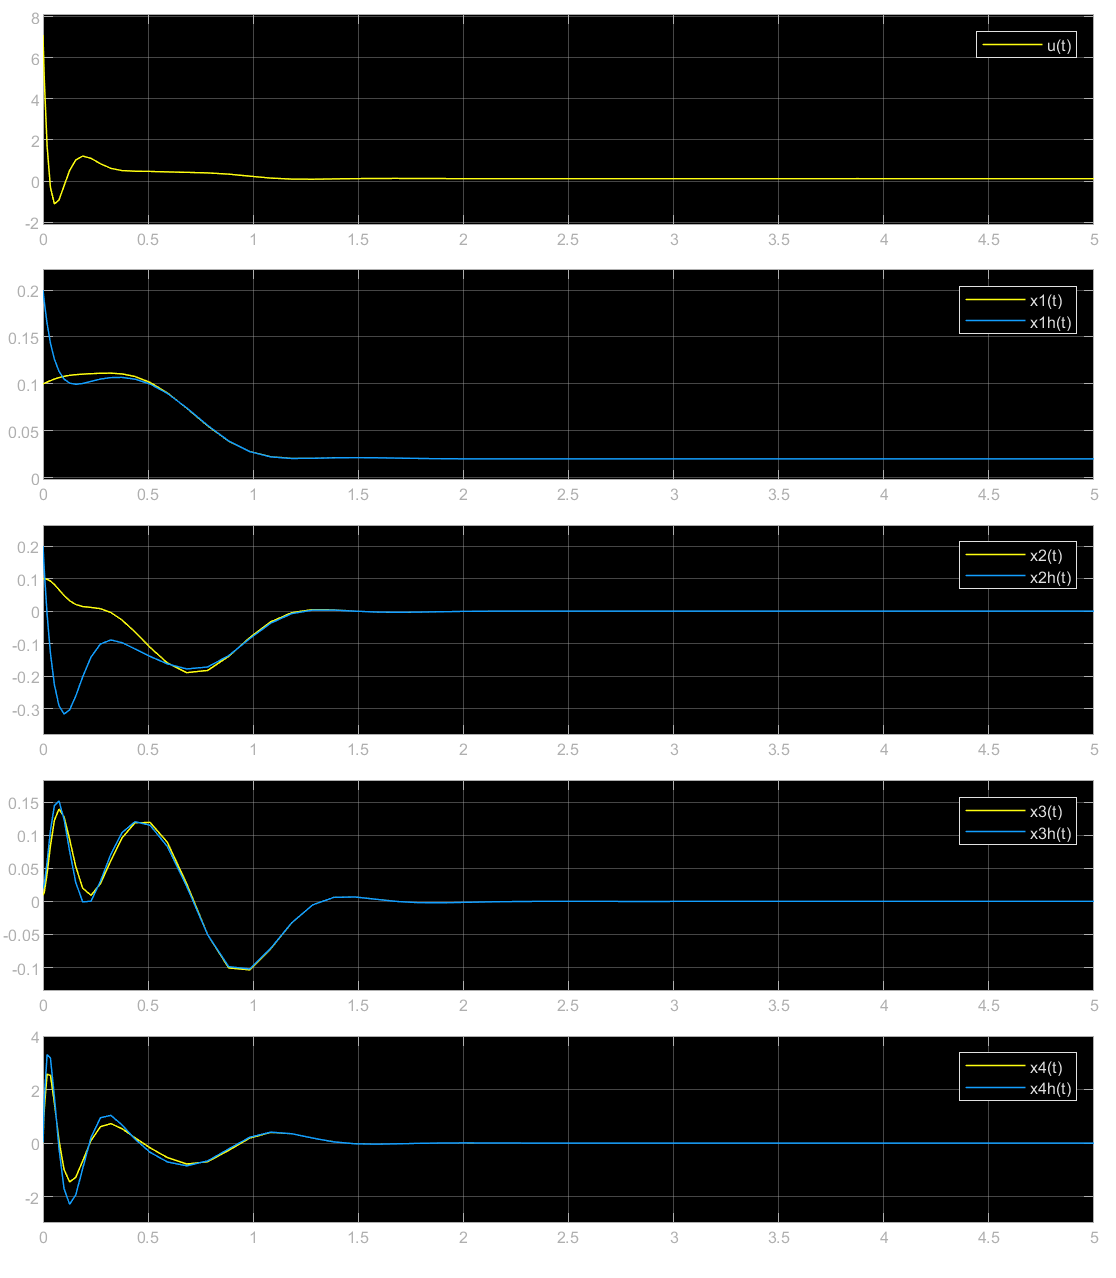
\includegraphics[width=\textwidth]{../images/m5_r0.02_s0.1_o0.2.png}
            \caption{$x_1(0) = x_2(0) = 0.1$ et $\hat{x}_1(0) = \hat{x}_2(0) = 0.2$}
        \end{subfigure}
        \begin{subfigure}[b]{0.475\textwidth}
            \centering
            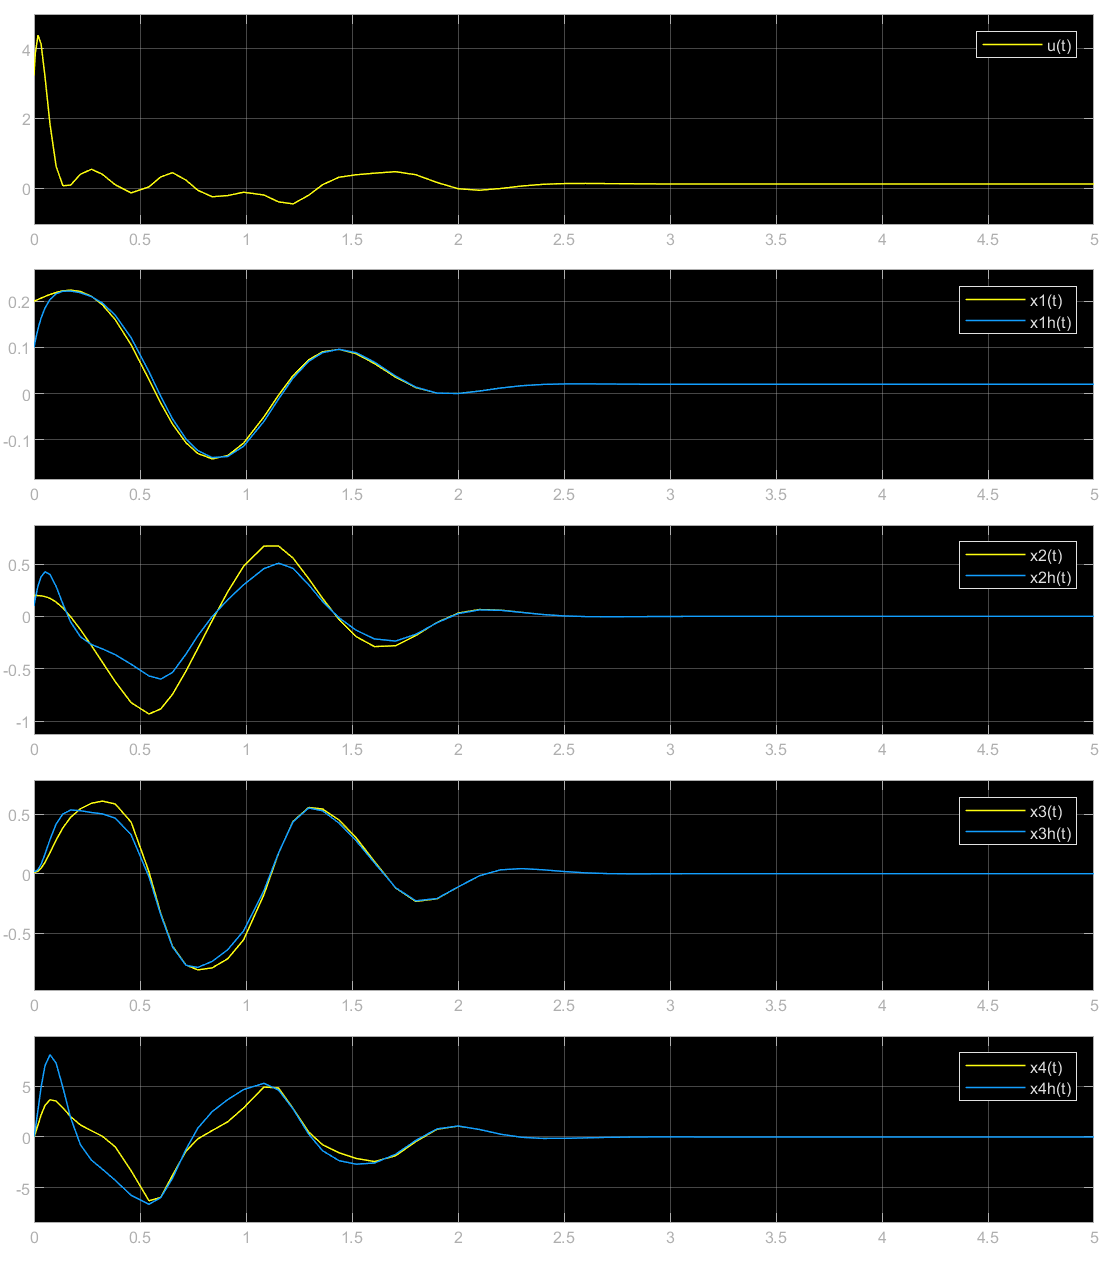
\includegraphics[width=\textwidth]{../images/m5_r0.02_s0.2_o0.1.png}
            \caption{$x_1(0) = x_2(0) = 0.2$ et $\hat{x}_1(0) = \hat{x}_2(0) = 0.1$}
        \end{subfigure}
        \caption{Simulation Observateur-Contrôleur, autour de $r_{\text{ref}} = 0.02$}
    \end{figure}
    On considère $x_3(0) = x_4(0) = 0.01$ et $\hat{x}_3(0) = \hat{x}_4(0) = 0.02$, un configuration où est possible stabiliser la Balle sur la position désirée donc la linéarisation est valable.
\end{resolution}

\newpage
\subsection{Question 25}
\begin{exercise}
    L'observateur-contrôleur est-il toujours performant lorsque la Balle s'éloigne significativement de la position $r_{\text{ref}} = 0$?
\end{exercise}
\begin{resolution}
    \begin{figure}[H]
        \centering
        \begin{subfigure}[b]{0.475\textwidth}
            \centering
            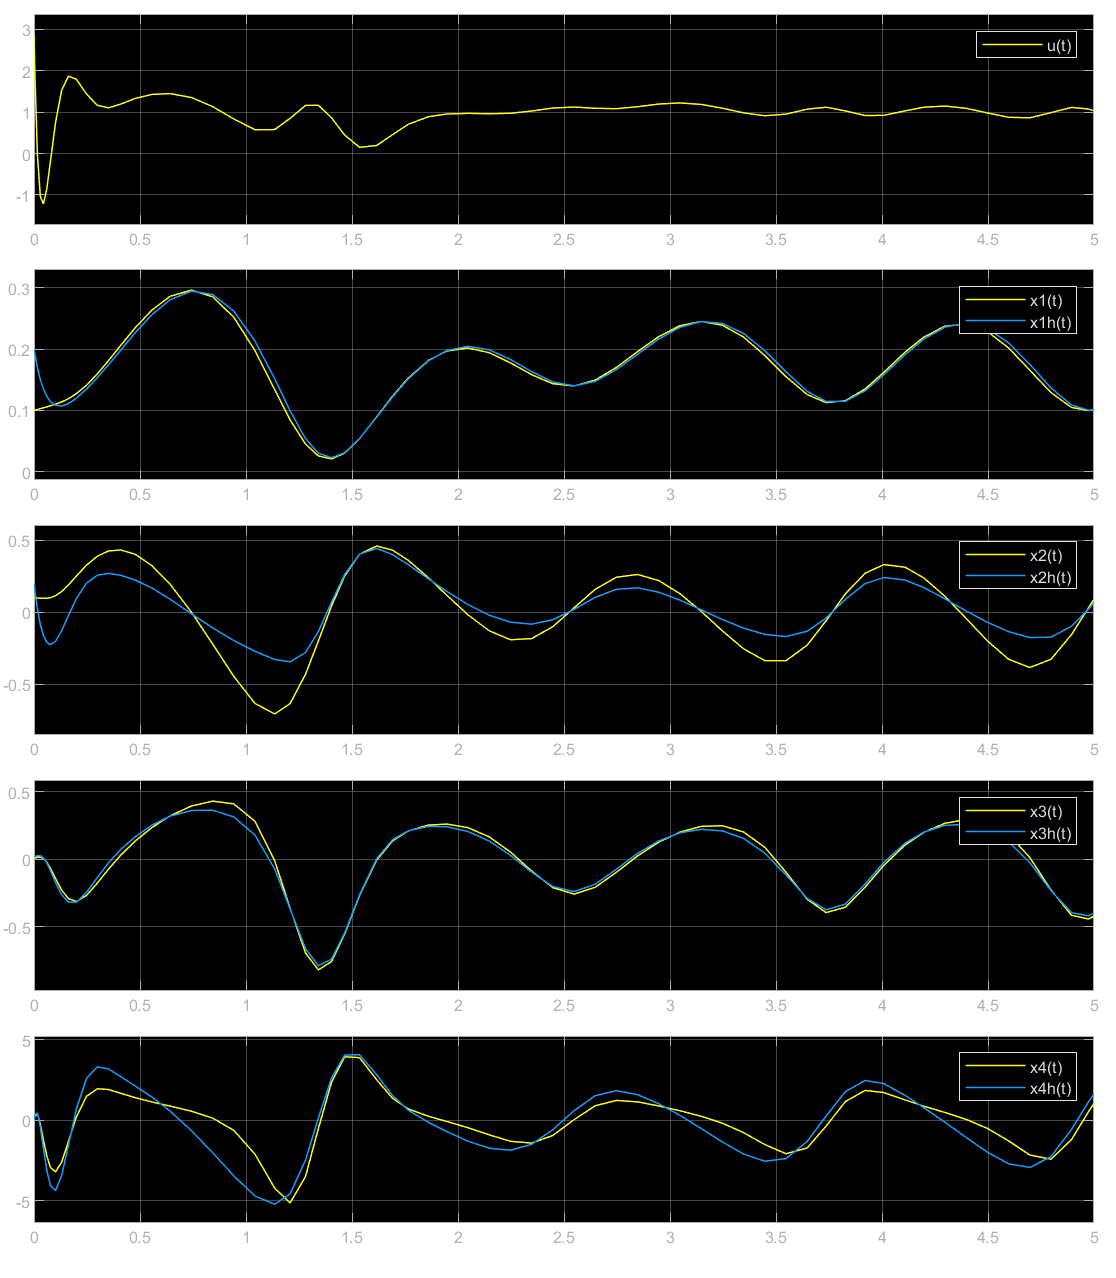
\includegraphics[width=\textwidth]{../images/m5_r0.2_s0.1_o0.2.png}
            \caption{$x_1(0) = x_2(0) = 0.1$ et $\hat{x}_1(0) = \hat{x}_2(0) = 0.2$}
        \end{subfigure}
        \begin{subfigure}[b]{0.475\textwidth}
            \centering
            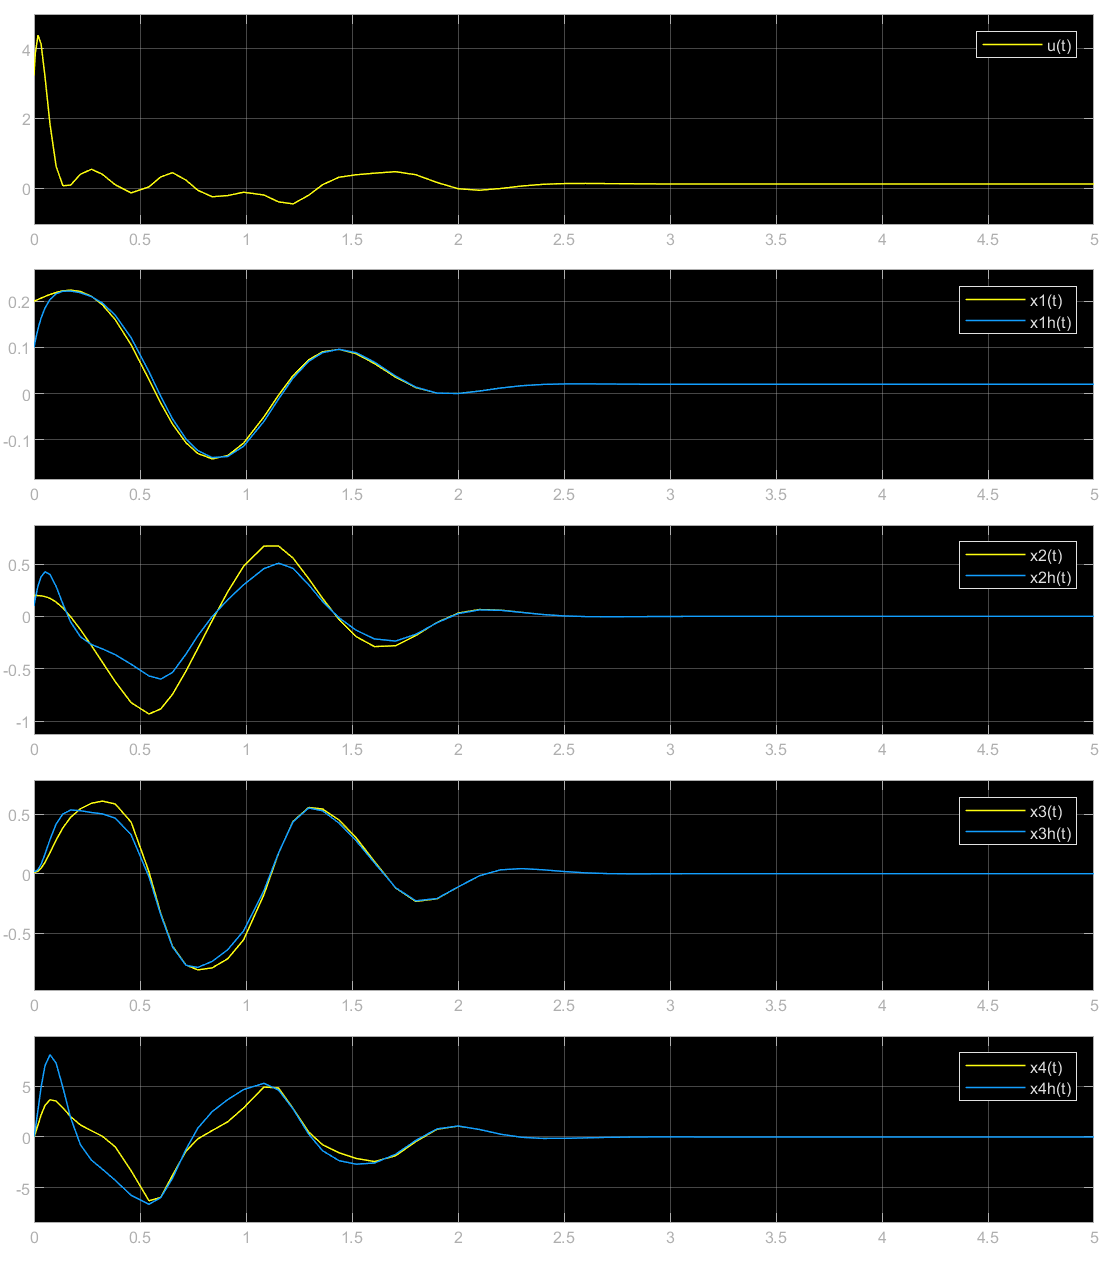
\includegraphics[width=\textwidth]{../images/m5_r0.02_s0.2_o0.1.png}
            \caption{$x_1(0) = x_2(0) = 0.2$ et $\hat{x}_1(0) = \hat{x}_2(0) = 0.1$}
        \end{subfigure}
        \caption{Simulation Observateur-Contrôleur, autour de $r_{\text{ref}} = 0.2$}
    \end{figure}
    On considère $x_3(0) = x_4(0) = 0.01$ et $\hat{x}_3(0) = \hat{x}_4(0) = 0.2$ qui fait que la Balle reste en oscillation autour du point d'équilibre désirée quand $x_1(0) \neq r_{\text{ref}}$ car la linéarisation n'est plus valable.\\
    
    Le Observateur-Contrôleur arrive a compenser le movement en dehors de la région considère mais c'est pas suffisamment, donc la Balle dépasse le point désirée et un comportement cyclique commence.\\

    Par contre, si $x_1(0) = r_{\text{ref}}$ le Observateur-Contrôleur arrive a stabiliser le système car il est déjà sur la région d'équilibre et donc la stabilisation est possible.
\end{resolution}
\end{document}